% Options for packages loaded elsewhere
\PassOptionsToPackage{unicode}{hyperref}
\PassOptionsToPackage{hyphens}{url}
\PassOptionsToPackage{dvipsnames,svgnames,x11names}{xcolor}
%
\documentclass[
  11pt,
]{article}

\usepackage{amsmath,amssymb}
\usepackage{setspace}
\usepackage{iftex}
\ifPDFTeX
  \usepackage[T1]{fontenc}
  \usepackage[utf8]{inputenc}
  \usepackage{textcomp} % provide euro and other symbols
\else % if luatex or xetex
  \usepackage{unicode-math}
  \defaultfontfeatures{Scale=MatchLowercase}
  \defaultfontfeatures[\rmfamily]{Ligatures=TeX,Scale=1}
\fi
\usepackage{lmodern}
\ifPDFTeX\else  
    % xetex/luatex font selection
\fi
% Use upquote if available, for straight quotes in verbatim environments
\IfFileExists{upquote.sty}{\usepackage{upquote}}{}
\IfFileExists{microtype.sty}{% use microtype if available
  \usepackage[]{microtype}
  \UseMicrotypeSet[protrusion]{basicmath} % disable protrusion for tt fonts
}{}
\makeatletter
\@ifundefined{KOMAClassName}{% if non-KOMA class
  \IfFileExists{parskip.sty}{%
    \usepackage{parskip}
  }{% else
    \setlength{\parindent}{0pt}
    \setlength{\parskip}{6pt plus 2pt minus 1pt}}
}{% if KOMA class
  \KOMAoptions{parskip=half}}
\makeatother
\usepackage{xcolor}
\usepackage[margin=1in]{geometry}
\setlength{\emergencystretch}{3em} % prevent overfull lines
\setcounter{secnumdepth}{5}
% Make \paragraph and \subparagraph free-standing
\makeatletter
\ifx\paragraph\undefined\else
  \let\oldparagraph\paragraph
  \renewcommand{\paragraph}{
    \@ifstar
      \xxxParagraphStar
      \xxxParagraphNoStar
  }
  \newcommand{\xxxParagraphStar}[1]{\oldparagraph*{#1}\mbox{}}
  \newcommand{\xxxParagraphNoStar}[1]{\oldparagraph{#1}\mbox{}}
\fi
\ifx\subparagraph\undefined\else
  \let\oldsubparagraph\subparagraph
  \renewcommand{\subparagraph}{
    \@ifstar
      \xxxSubParagraphStar
      \xxxSubParagraphNoStar
  }
  \newcommand{\xxxSubParagraphStar}[1]{\oldsubparagraph*{#1}\mbox{}}
  \newcommand{\xxxSubParagraphNoStar}[1]{\oldsubparagraph{#1}\mbox{}}
\fi
\makeatother


\providecommand{\tightlist}{%
  \setlength{\itemsep}{0pt}\setlength{\parskip}{0pt}}\usepackage{longtable,booktabs,array}
\usepackage{calc} % for calculating minipage widths
% Correct order of tables after \paragraph or \subparagraph
\usepackage{etoolbox}
\makeatletter
\patchcmd\longtable{\par}{\if@noskipsec\mbox{}\fi\par}{}{}
\makeatother
% Allow footnotes in longtable head/foot
\IfFileExists{footnotehyper.sty}{\usepackage{footnotehyper}}{\usepackage{footnote}}
\makesavenoteenv{longtable}
\usepackage{graphicx}
\makeatletter
\def\maxwidth{\ifdim\Gin@nat@width>\linewidth\linewidth\else\Gin@nat@width\fi}
\def\maxheight{\ifdim\Gin@nat@height>\textheight\textheight\else\Gin@nat@height\fi}
\makeatother
% Scale images if necessary, so that they will not overflow the page
% margins by default, and it is still possible to overwrite the defaults
% using explicit options in \includegraphics[width, height, ...]{}
\setkeys{Gin}{width=\maxwidth,height=\maxheight,keepaspectratio}
% Set default figure placement to htbp
\makeatletter
\def\fps@figure{htbp}
\makeatother

\usepackage{hyperref}
\usepackage{float}
\hypersetup{
  colorlinks=true,
  linkcolor=blue,
  urlcolor=blue,
  breaklinks=true,
  pdfborder={0 0 0}
}
\makeatletter
\@ifpackageloaded{caption}{}{\usepackage{caption}}
\AtBeginDocument{%
\ifdefined\contentsname
  \renewcommand*\contentsname{Table of contents}
\else
  \newcommand\contentsname{Table of contents}
\fi
\ifdefined\listfigurename
  \renewcommand*\listfigurename{List of Figures}
\else
  \newcommand\listfigurename{List of Figures}
\fi
\ifdefined\listtablename
  \renewcommand*\listtablename{List of Tables}
\else
  \newcommand\listtablename{List of Tables}
\fi
\ifdefined\figurename
  \renewcommand*\figurename{Figure}
\else
  \newcommand\figurename{Figure}
\fi
\ifdefined\tablename
  \renewcommand*\tablename{Table}
\else
  \newcommand\tablename{Table}
\fi
}
\@ifpackageloaded{float}{}{\usepackage{float}}
\floatstyle{ruled}
\@ifundefined{c@chapter}{\newfloat{codelisting}{h}{lop}}{\newfloat{codelisting}{h}{lop}[chapter]}
\floatname{codelisting}{Listing}
\newcommand*\listoflistings{\listof{codelisting}{List of Listings}}
\makeatother
\makeatletter
\makeatother
\makeatletter
\@ifpackageloaded{caption}{}{\usepackage{caption}}
\@ifpackageloaded{subcaption}{}{\usepackage{subcaption}}
\makeatother
\ifLuaTeX
  \usepackage{selnolig}  % disable illegal ligatures
\fi
\usepackage[]{biblatex}
\addbibresource{references.bib}
\usepackage{bookmark}

\IfFileExists{xurl.sty}{\usepackage{xurl}}{} % add URL line breaks if available
\urlstyle{same} % disable monospaced font for URLs
\hypersetup{
  pdftitle={William's Update},
  pdfauthor={William Clinton Co},
  colorlinks=true,
  linkcolor={blue},
  filecolor={Maroon},
  citecolor={blue},
  urlcolor={blue},
  pdfcreator={LaTeX via pandoc}}

\title{William's Update}
\usepackage{etoolbox}
\makeatletter
\providecommand{\subtitle}[1]{% add subtitle to \maketitle
  \apptocmd{\@title}{\par {\large #1 \par}}{}{}
}
\makeatother
\subtitle{Remittances}
\author{William Clinton Co}
\date{September 12, 2025}

\begin{document}
\maketitle
\begin{abstract}
This document is a follow-up to the meeting on September 29th and
addresses the items discussed during that meeting. This provides an
update on who was contacted regarding the remittance datasets, offers
updates on previously problematic pdf file links, and clarifies how the
stablecoin/bitcoin cross-border flows dataset works. Most importantly,
this presents the extracted remittance data from Remitscope.
\end{abstract}

\renewcommand*\contentsname{Table of contents}
{
\hypersetup{linkcolor=}
\setcounter{tocdepth}{10}
\tableofcontents
}
\setstretch{1}
\section{Data Update}\label{data-update}

I have contacted two authors from
\href{https://www.imf.org/en/Publications/WP/Issues/2021/07/16/Defying-the-Odds-Remittances-During-the-COVID-19-Pandemic-461321}{Defying
the Odds: Remittances During the COVID-19 Pandemic}

\begin{itemize}
\tightlist
\item
  The Remitscope data is reliable but incomplete
\item
  \href{https://www.imf.org/en/Publications/WP/Issues/2021/07/16/Defying-the-Odds-Remittances-During-the-COVID-19-Pandemic-461321}{Defying
  the Odds: Remittances During the COVID-19 Pandemic} provides
  additional data to the Remitscope data.
\item
  I am currently waiting for access to their dataset so that we can
  merge their dataset (2018-2020) to ours (2019-2024)
\item
  It may be worth consideraing looking at each website ill work on that.
\end{itemize}

\section{Data Analysis Results}\label{data-analysis-results}

\subsection{Overview}\label{overview}

This analysis examines remittance flows using data extracted from
Remitscope, covering 728 remittance records from 2019-2024.

\subsubsection{Data Completeness
Summary}\label{data-completeness-summary}

\begin{itemize}
\tightlist
\item
  \textbf{Total records}: 728
\item
  \textbf{Date range}: 2019 - 2024
\item
  \textbf{Sending countries}: 206
\item
  \textbf{Receiving countries}: 20 (limited coverage - only 10.3\% of
  world)
\end{itemize}

\subsection{Interactive
Visualizations}\label{interactive-visualizations}

\subsection{Sending Countries
Analysis}\label{sending-countries-analysis}

The remittance data shows a global distribution of sending countries,
with developed nations dominating the top positions:

\subsubsection{Top 10 Sending Countries}\label{top-10-sending-countries}

\begin{verbatim}
Sending Country              Records
Canada                           18
Italy                           15  
United States of America        15
Spain                           14
France                          14
Germany                         14
United Kingdom                  12
China                           11
Sweden                          10
Switzerland                     10
\end{verbatim}

\subsection{Receiving Countries
Analysis}\label{receiving-countries-analysis}

The receiving countries show a strong concentration in Latin America:

\subsubsection{Top 10 Receiving
Countries}\label{top-10-receiving-countries}

\begin{verbatim}
Receiving Country           Records
Ecuador                        183
Mexico                         169  
Panama                         102
Senegal                         38
Kenya                           34
Colombia                        32
Uganda                          20
Chile                           19
Morocco                         19
Ethiopia                        17
\end{verbatim}

\subsection{Temporal Distribution}\label{temporal-distribution}

The data collection shows significant variation across years:

\subsubsection{Records by Year}\label{records-by-year}

\begin{figure}[H]

\centering{

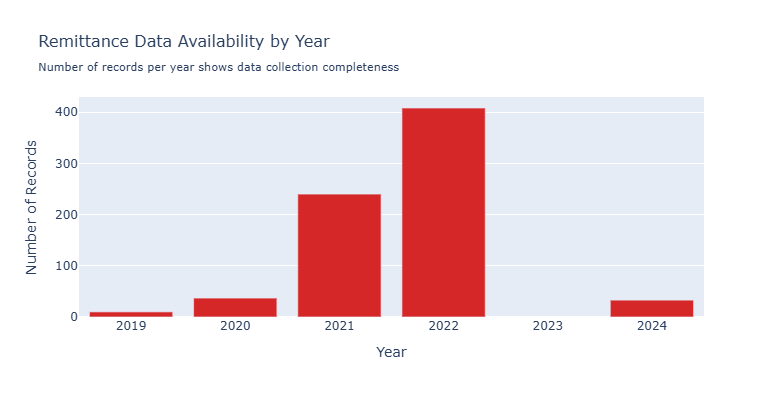
\includegraphics[width=1\textwidth,height=\textheight]{images/2.png}

}

\caption{\label{fig-records-by-year}Records by Year}

\end{figure}%

\textbf{Note}: 2023 data is completely missing from the dataset.

\subsection{Key Findings}\label{key-findings}

\begin{itemize}
\tightlist
\item
  \textbf{Peak Collection}: 2022 shows the highest data collection with
  408 records
\item
  \textbf{Geographic Concentration}:

  \begin{itemize}
  \tightlist
  \item
    \textbf{Sending}: Distributed globally across 206 countries
    (developed nations leading)
  \item
    \textbf{Receiving}: Highly concentrated with top 3 countries
    (Ecuador, Mexico, Panama) accounting for 454/728 records (62.4\%)
  \end{itemize}
\end{itemize}

Please access the HTML files in:
\href{https://github.com/WilliamClintC/RER/tree/main/_output/exported_figures}{\texttt{output\textbackslash{}exported\_figures\textbackslash{}}}

\section{Visual Analysis}\label{visual-analysis}

\subsection{Sending Countries
Analysis}\label{sending-countries-analysis-1}

\begin{figure}[H]

\centering{

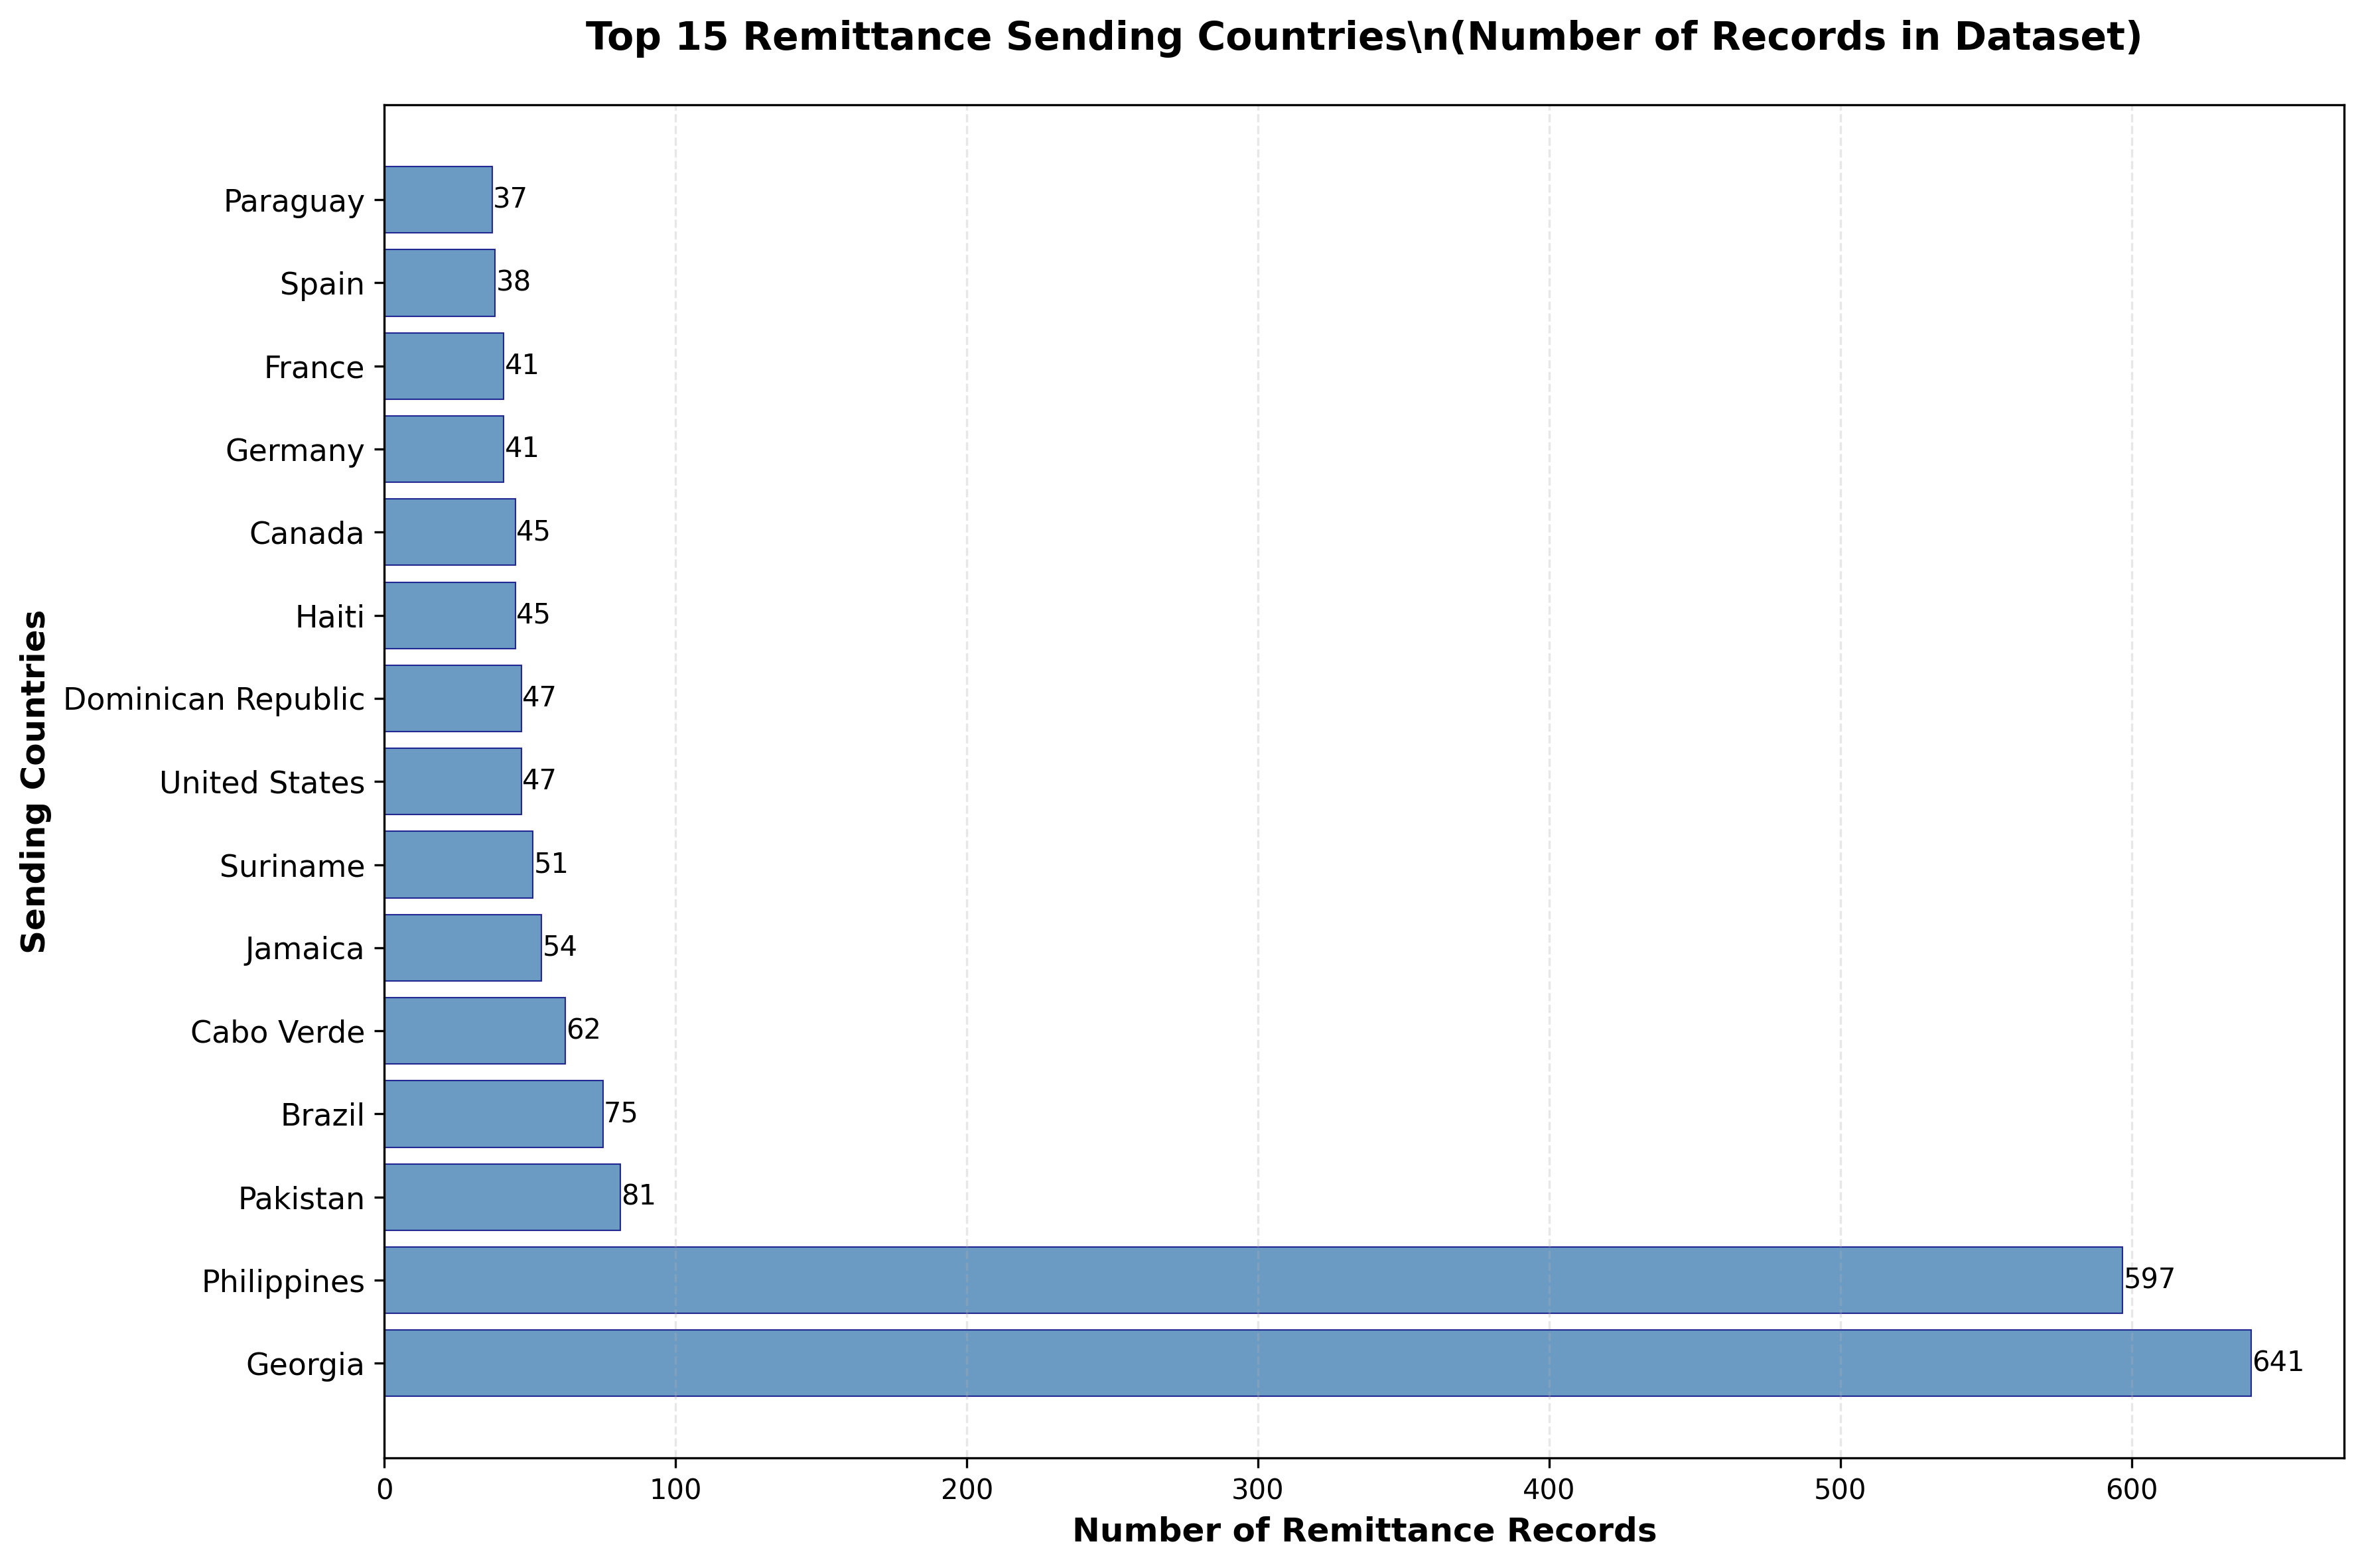
\includegraphics[width=1\textwidth,height=\textheight]{images/sending_countries_static.png}

}

\caption{\label{fig-sending-static}Top 15 Remittance Sending Countries}

\end{figure}%

\begin{figure}[H]

\centering{

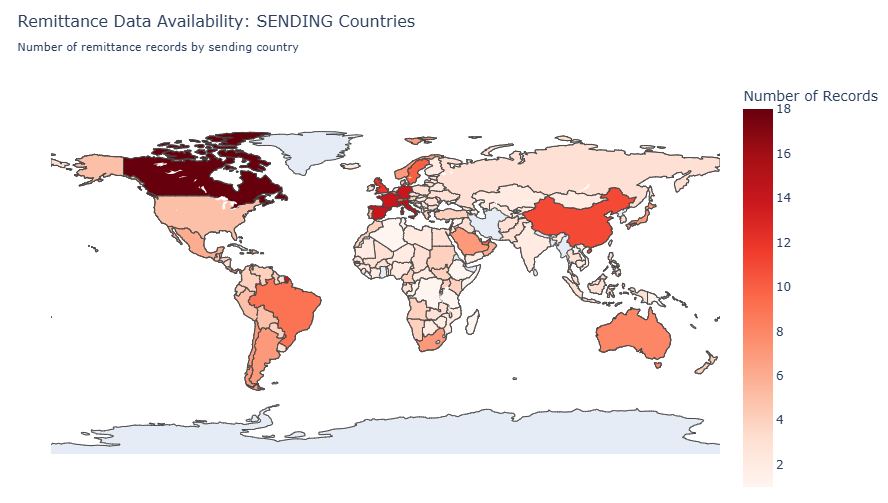
\includegraphics[width=1\textwidth,height=\textheight]{images/3.png}

}

\caption{\label{fig-sending-additional}Additional Sending Countries
Analysis}

\end{figure}%

The analysis reveals that developed nations dominate remittance sending,
with Canada leading at 18 records, followed by Italy, USA, Spain,
France, and Germany each contributing 14-15 records.

\begin{figure}[H]

\centering{

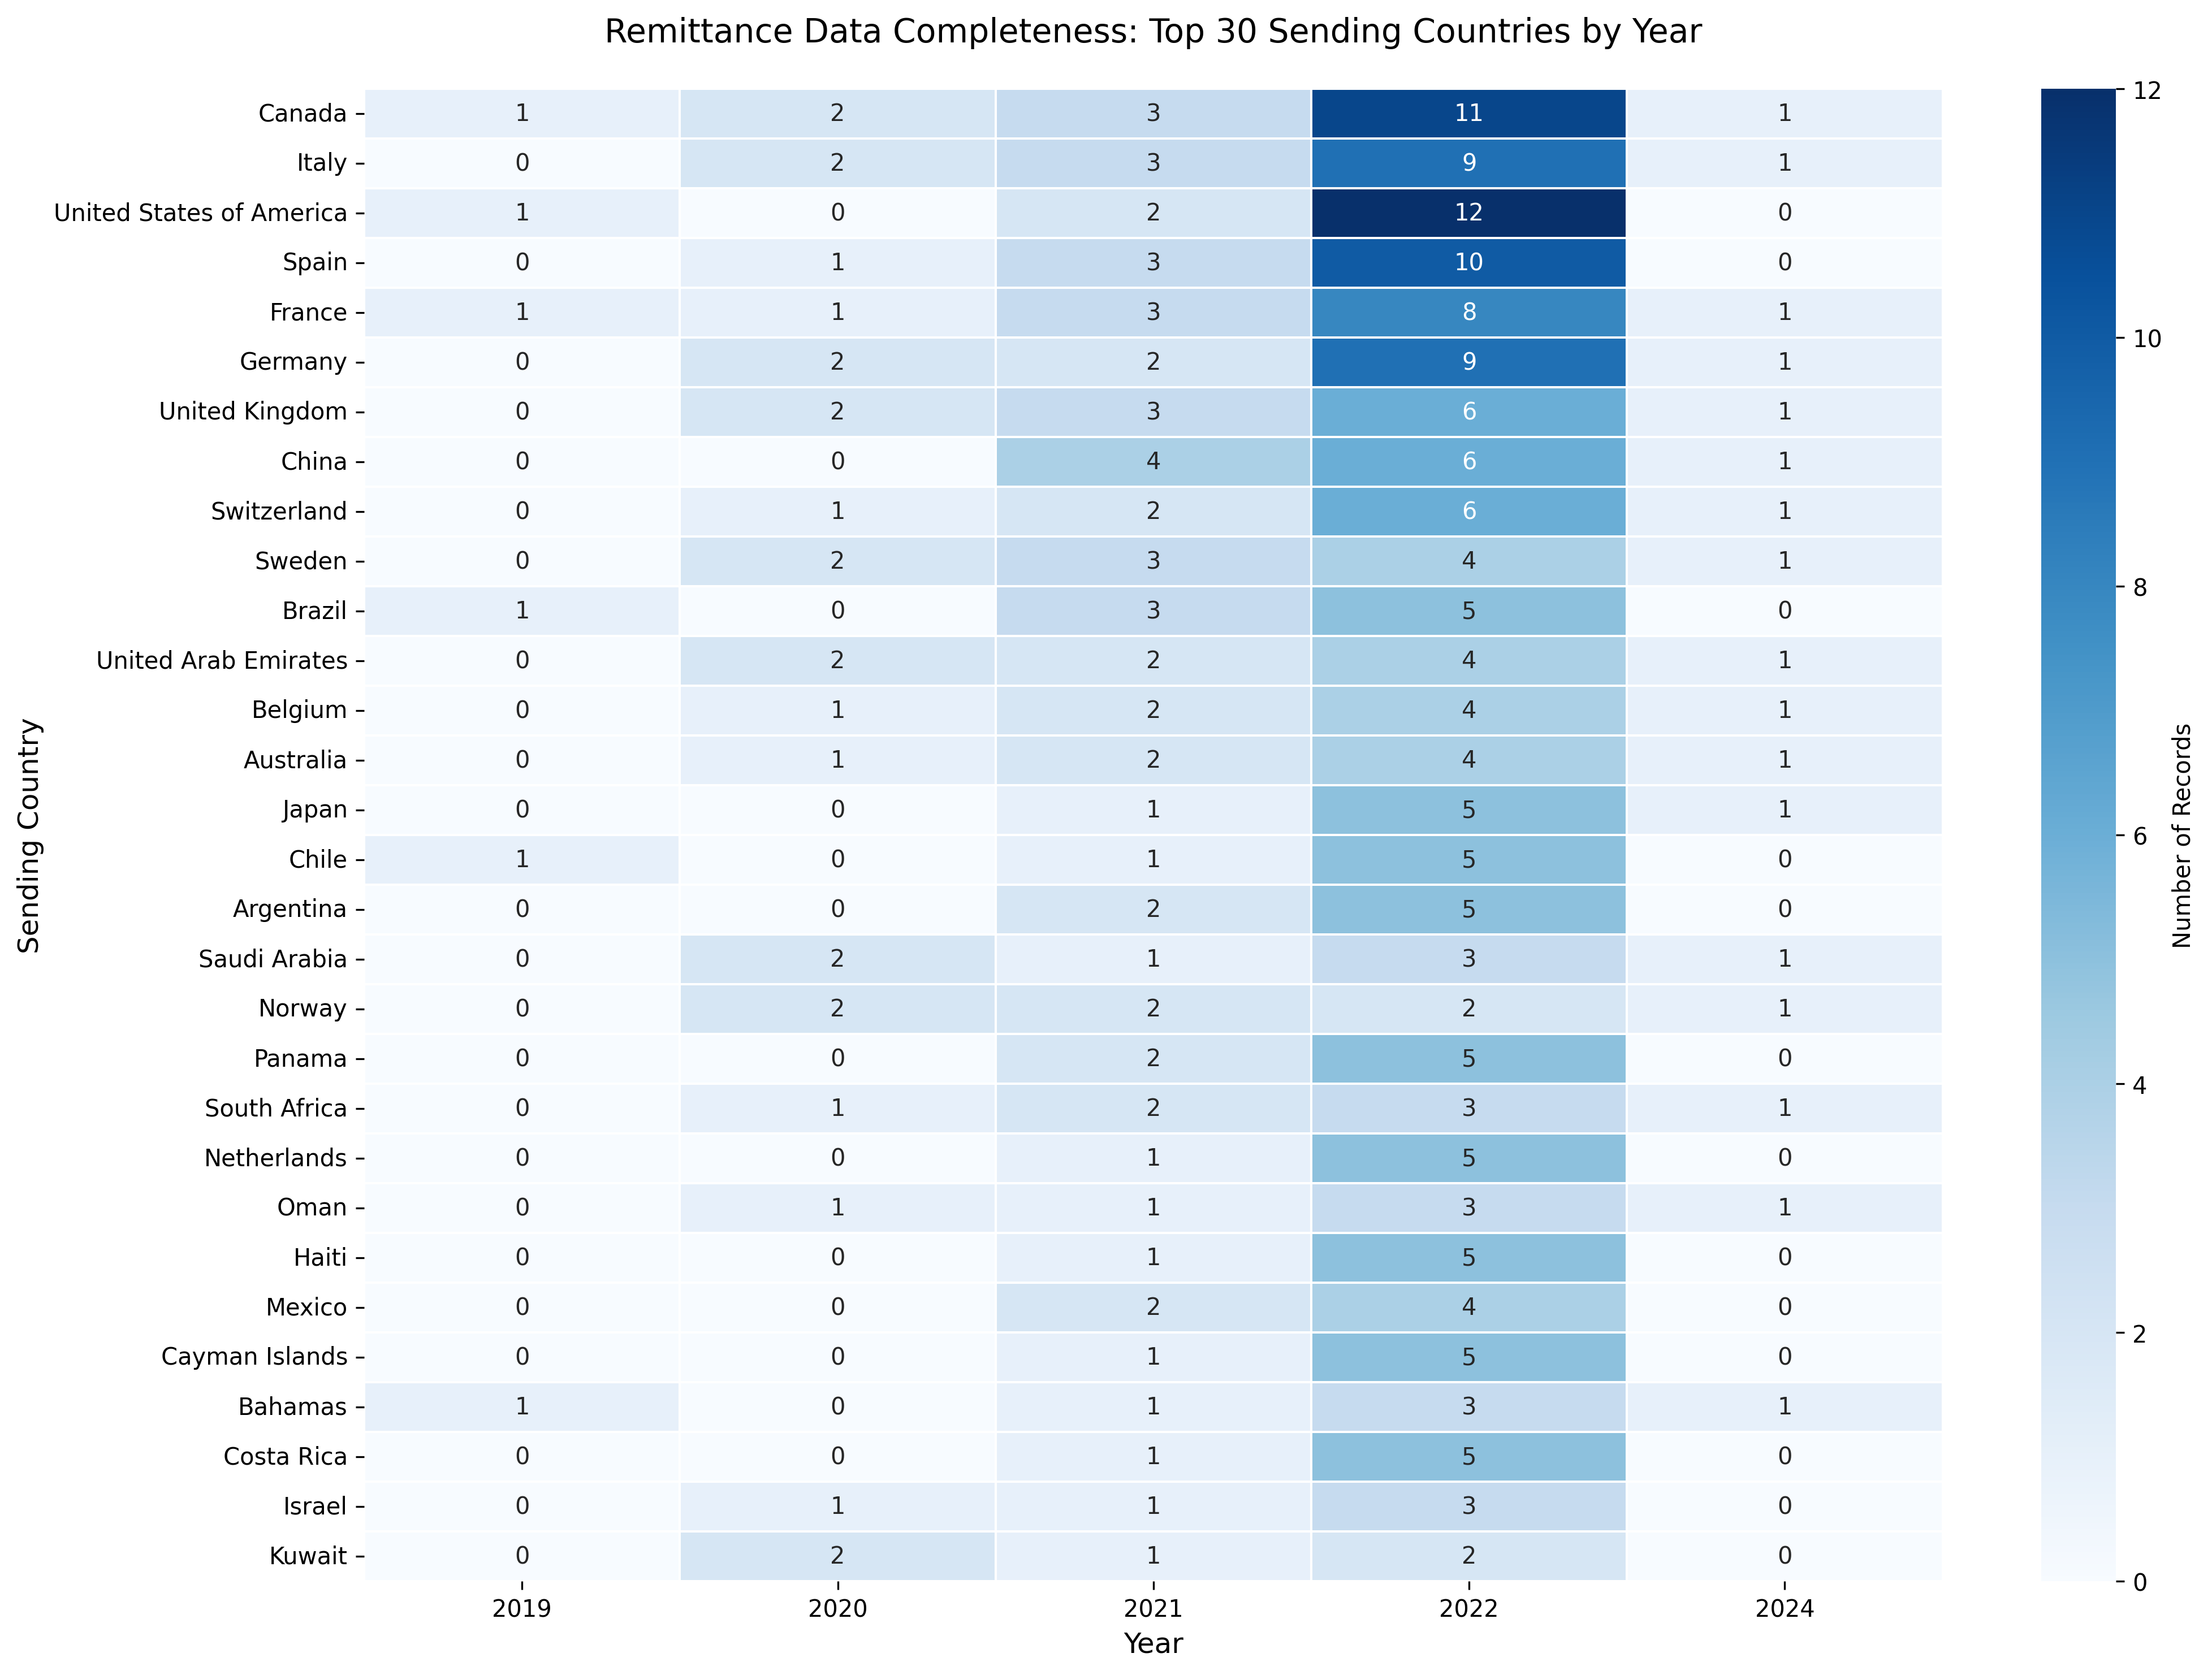
\includegraphics[width=1\textwidth,height=\textheight]{images/sending_heatmap.png}

}

\caption{\label{fig-sending-heatmap-detail}Sending Countries Temporal
Heatmap}

\end{figure}%

\subsubsection{Receiving Countries
Analysis}\label{receiving-countries-analysis-1}

\begin{figure}[H]

\centering{

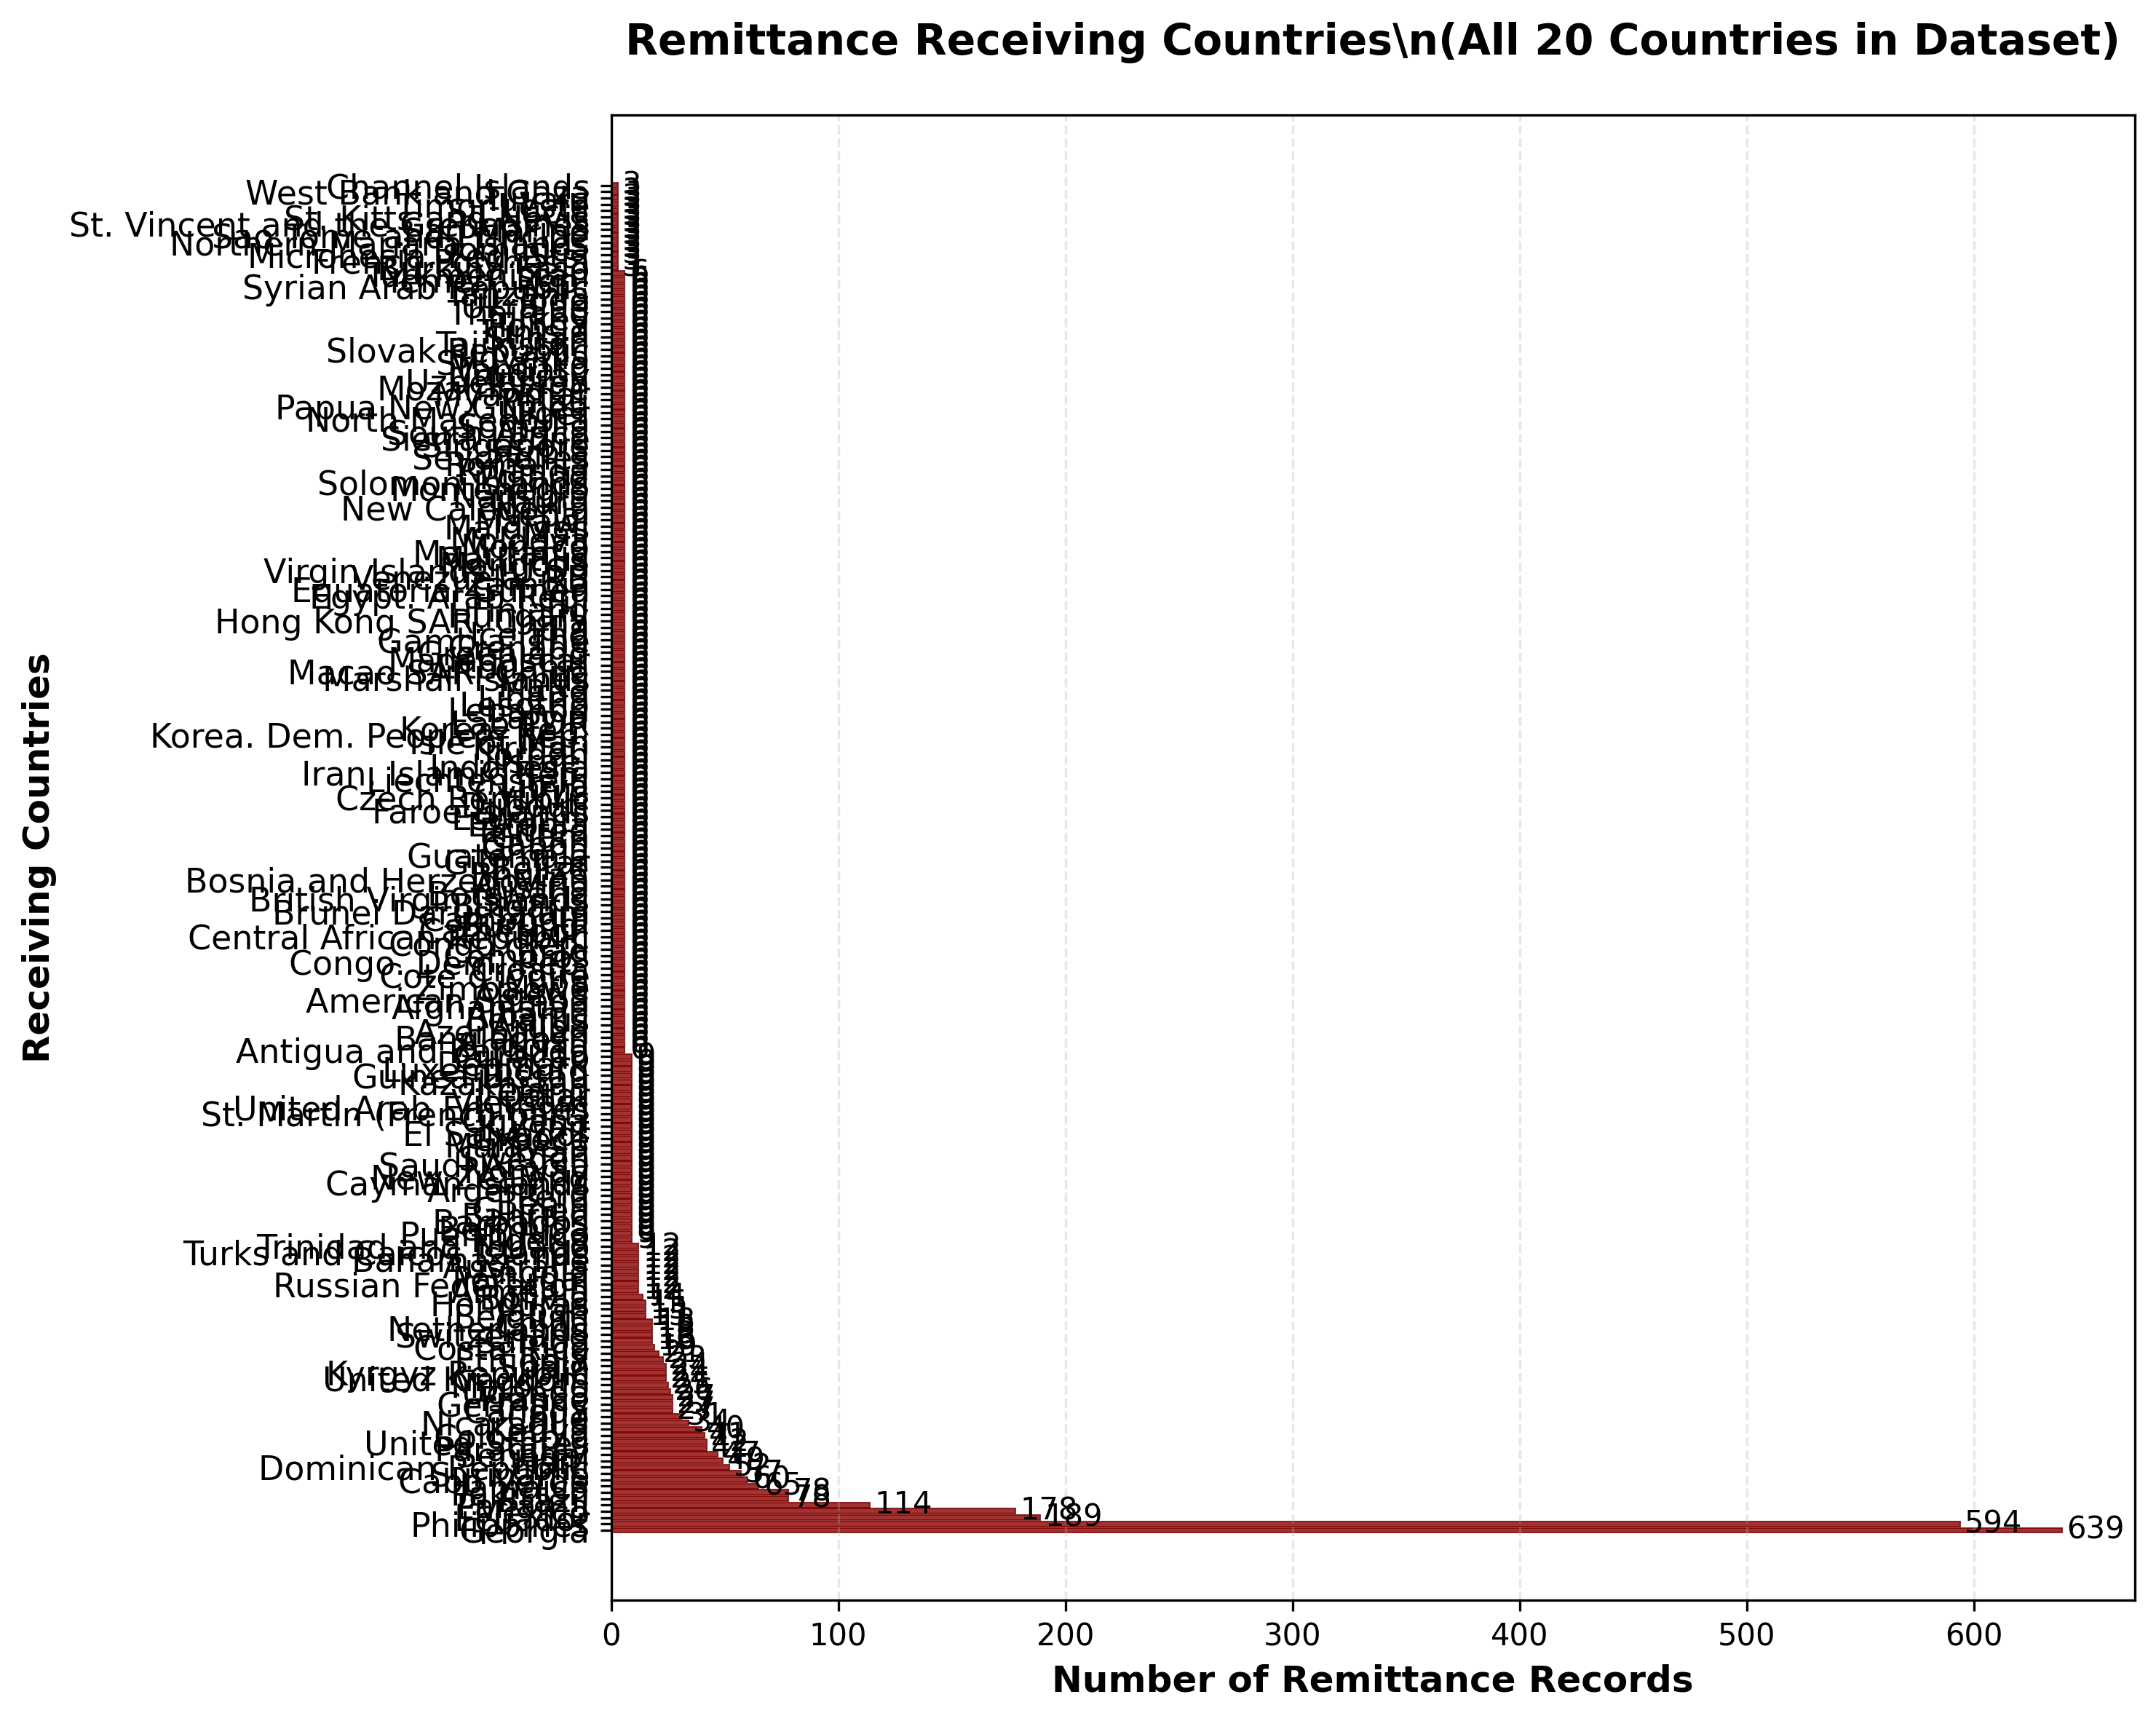
\includegraphics[width=1\textwidth,height=\textheight]{images/receiving_countries_static.png}

}

\caption{\label{fig-receiving-static}All 20 Remittance Receiving
Countries}

\end{figure}%

\begin{figure}[H]

\centering{

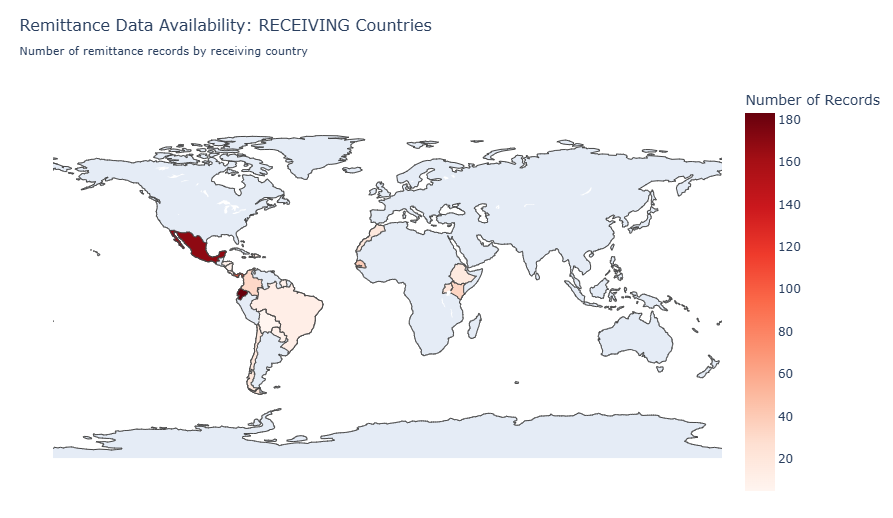
\includegraphics[width=1\textwidth,height=\textheight]{images/4.png}

}

\caption{\label{fig-receiving-additional}Additional Receiving Countries
Analysis}

\end{figure}%

The receiving countries show strong concentration in Latin America, with
Ecuador (183 records) and Mexico (169 records) dominating the dataset.

\begin{figure}[H]

\centering{

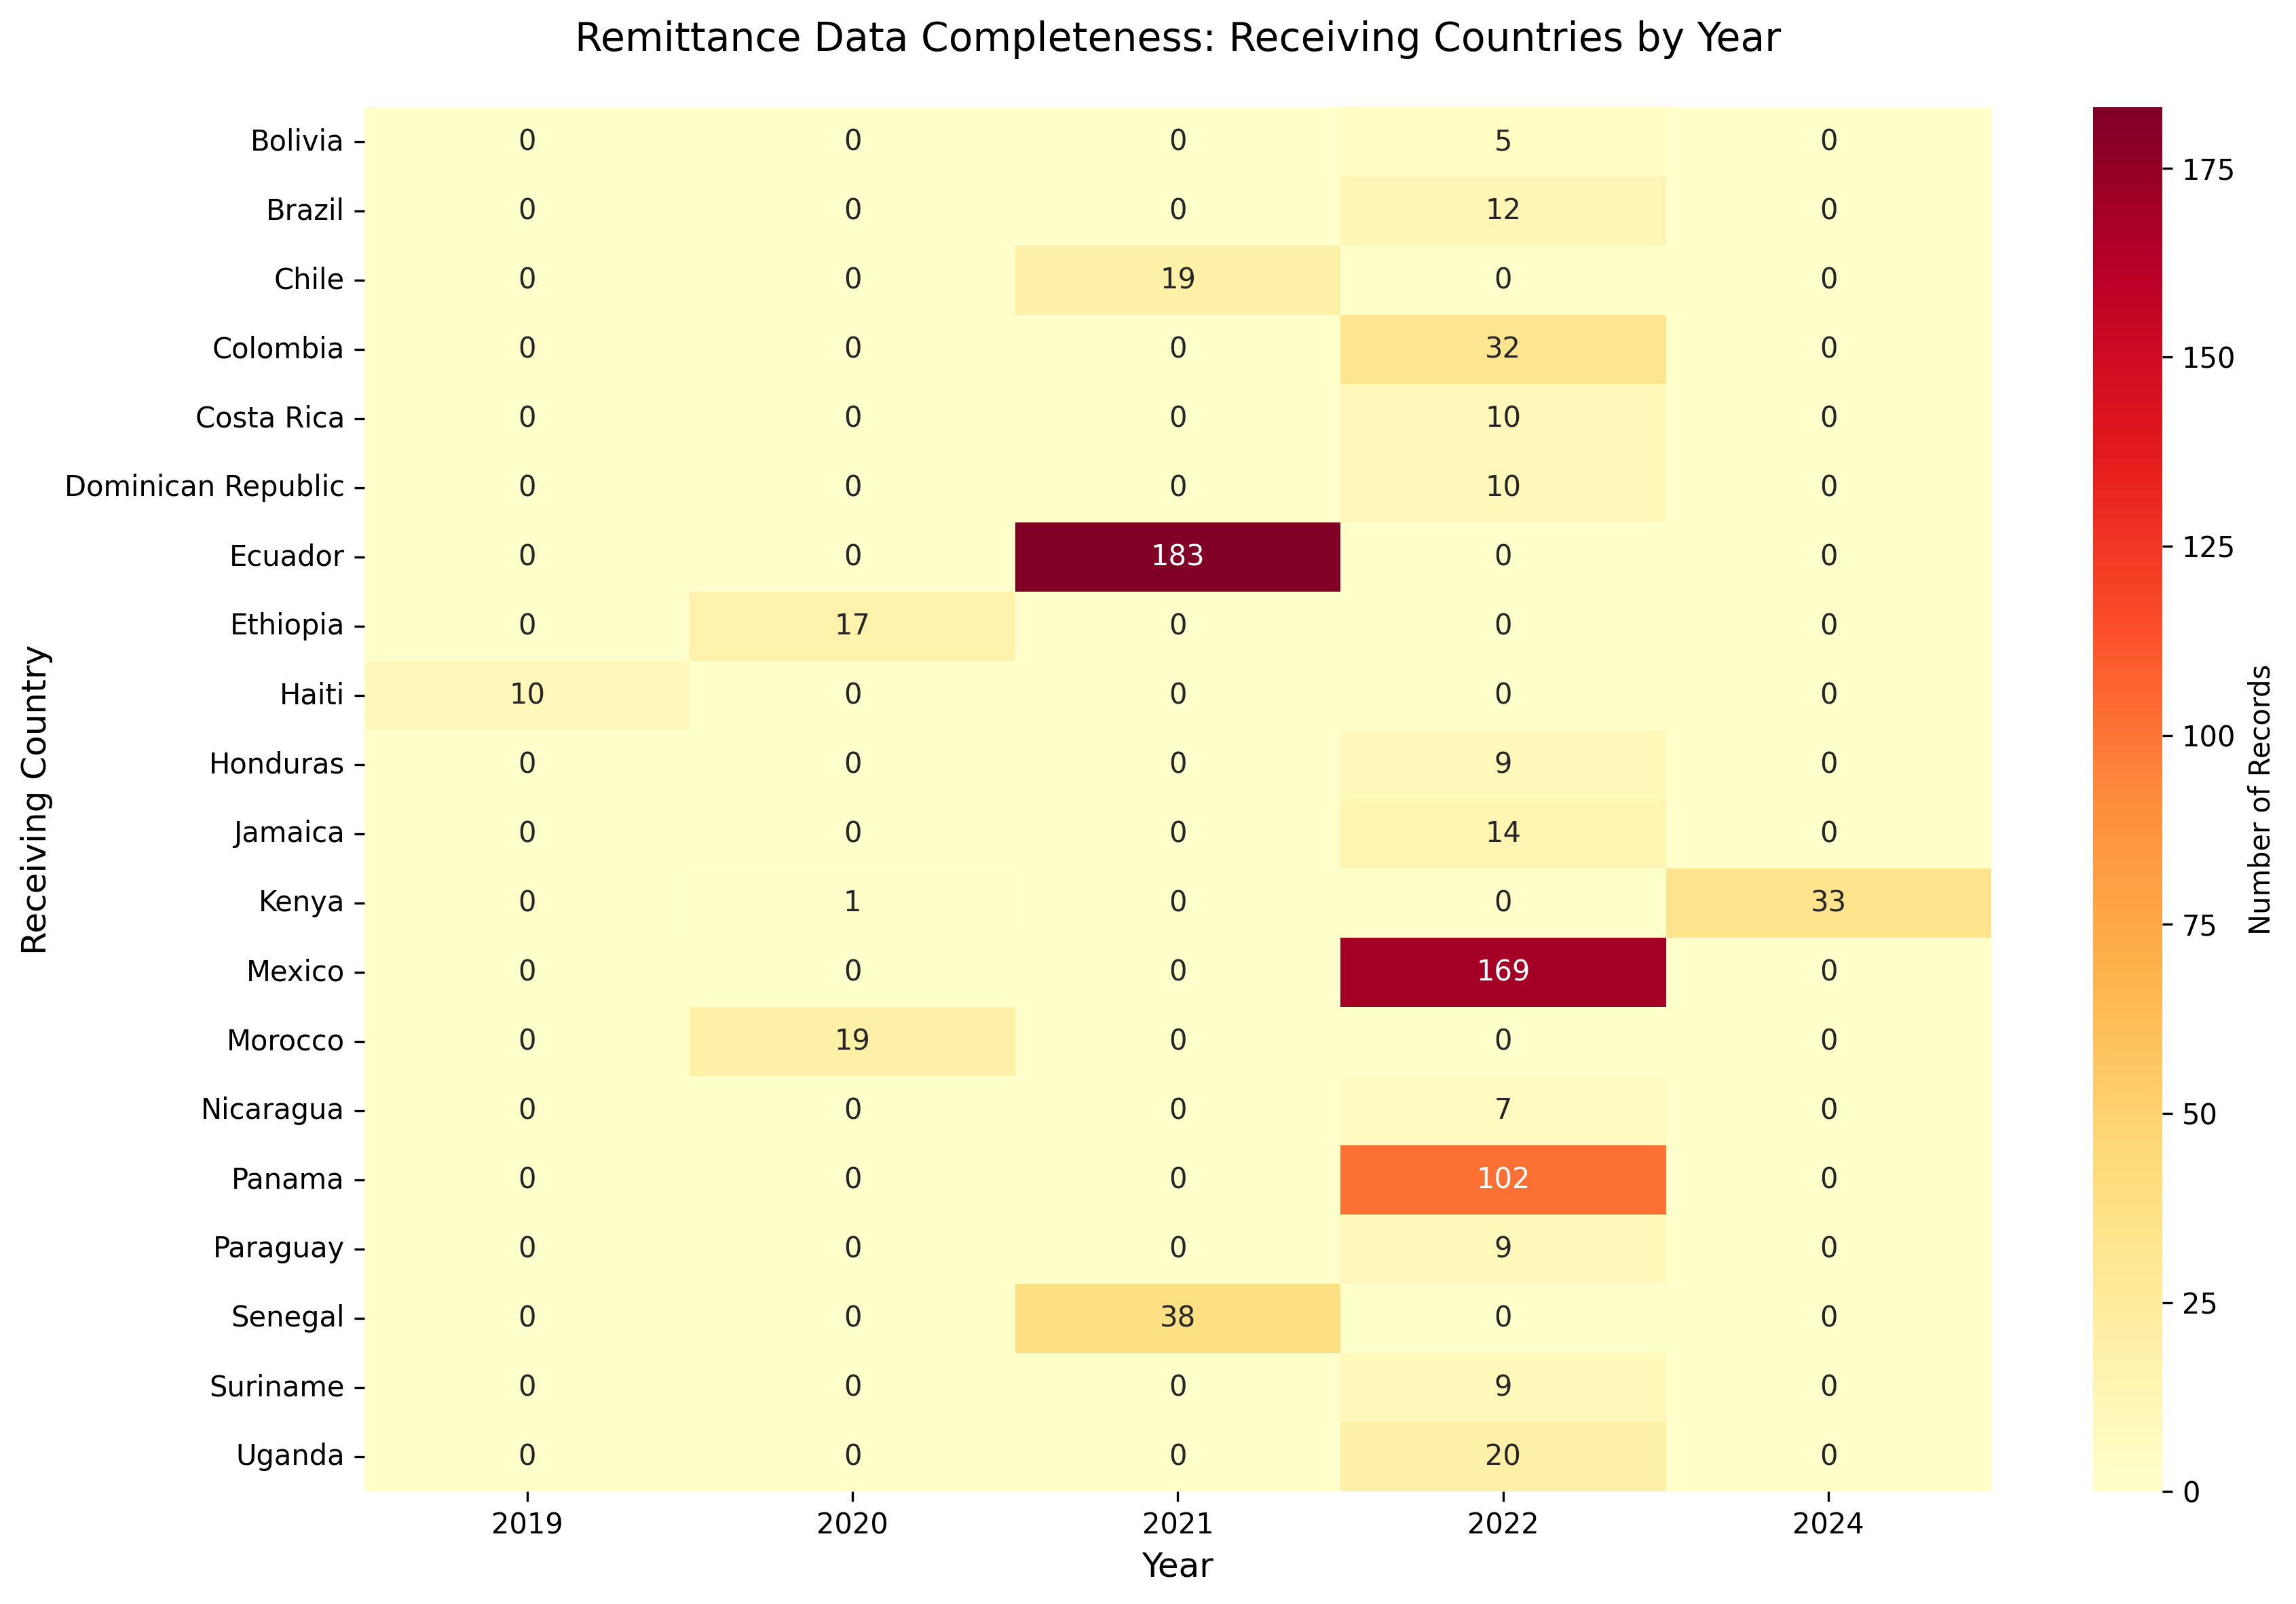
\includegraphics[width=1\textwidth,height=\textheight]{images/receiving_heatmap.png}

}

\caption{\label{fig-receiving-heatmap-detail}Receiving Countries
Temporal Heatmap Detail}

\end{figure}%

\subsection{Data concentration:}\label{data-concentration}

\begin{itemize}
\tightlist
\item
  Top 10 receiving countries: 633/728 records (87.0\%)
\item
  Top 10 sending countries: 133/728 records (18.3\%)
\end{itemize}

\subsection{Main Flows}\label{main-flows}

\begin{figure}[H]

\centering{

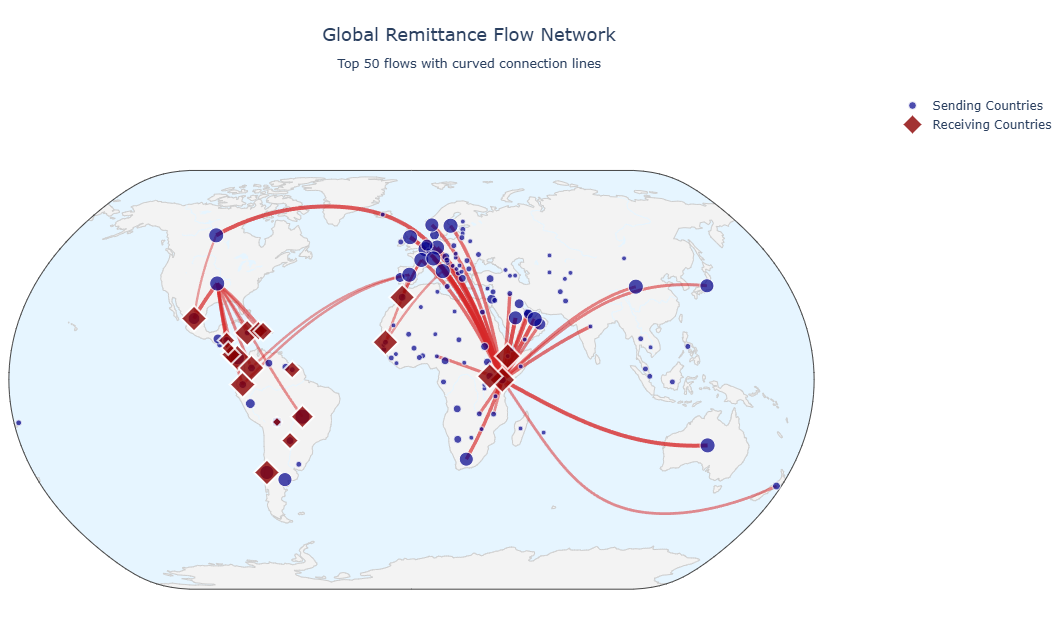
\includegraphics[width=1\textwidth,height=\textheight]{images/5.png}

}

\caption{\label{fig-main-flows}Main Remittance Flow Patterns}

\end{figure}%

\textbf{Interactive HTML Link}:
\href{https://github.com/WilliamClintC/RER/blob/main/_output/exported_figures/04_initial_flow_map_top50.html}{View
Interactive Main Flow Map}

\subsection{Complete Flows}\label{complete-flows}

\begin{figure}[H]

\centering{

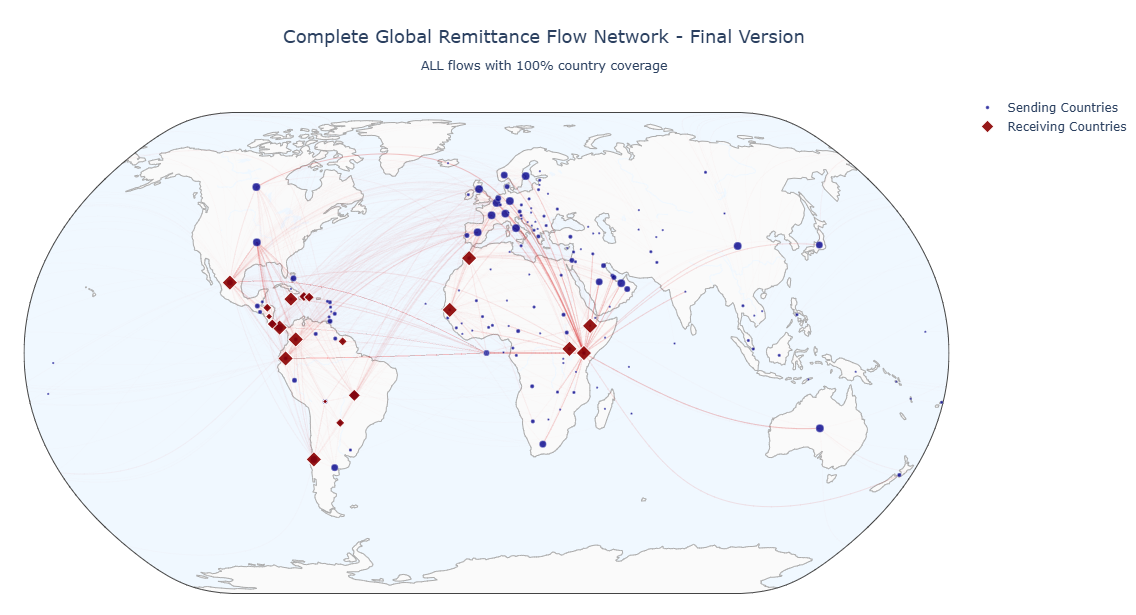
\includegraphics[width=1\textwidth,height=\textheight]{images/7.png}

}

\caption{\label{fig-complete-flows}Complete Remittance Flow Coverage}

\end{figure}%

\textbf{Interactive HTML Link}:
\href{https://github.com/WilliamClintC/RER/blob/main/_output/exported_figures/07_final_flow_map_100percent_coverage.html}{View
Interactive Complete Flow Map}

\subsection{Complete Flows with Small Flows
Visibility}\label{complete-flows-with-small-flows-visibility}

\begin{figure}[H]

\centering{

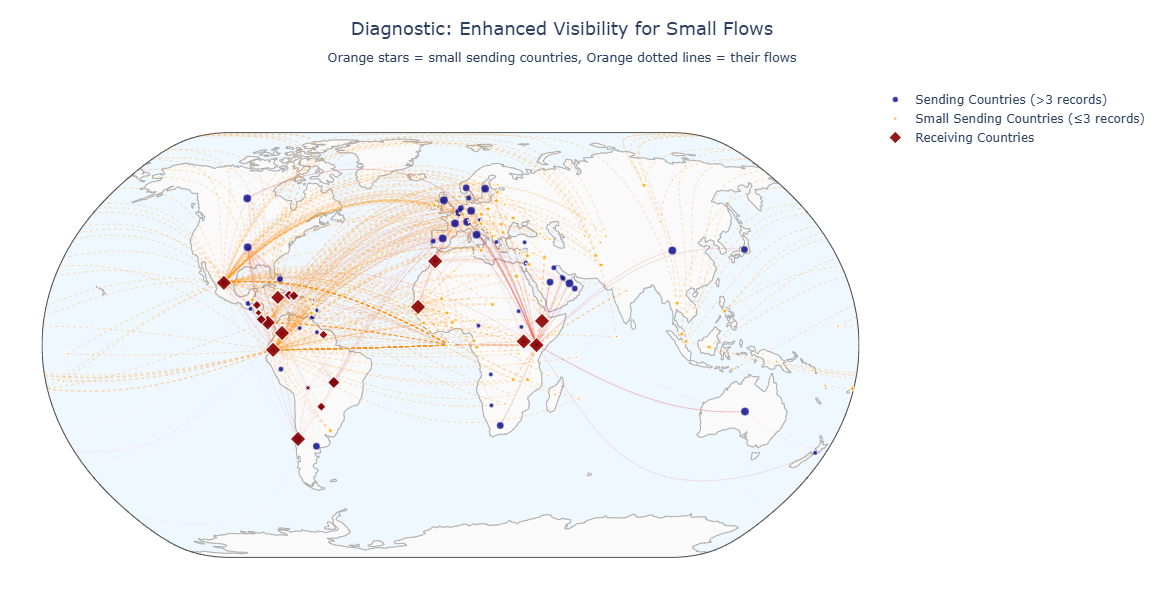
\includegraphics[width=1\textwidth,height=\textheight]{images/8.png}

}

\caption{\label{fig-enhanced-visibility}Enhanced Visibility for Small
Flows}

\end{figure}%

\textbf{Interactive HTML Link}:
\href{https://github.com/WilliamClintC/RER/blob/main/_output/exported_figures/08_diagnostic_enhanced_visibility.html}{View
Interactive Enhanced Visibility Map}

\subsection{Main Flow vs Complete Flow
Comparison}\label{main-flow-vs-complete-flow-comparison}

\begin{figure}[H]

\centering{

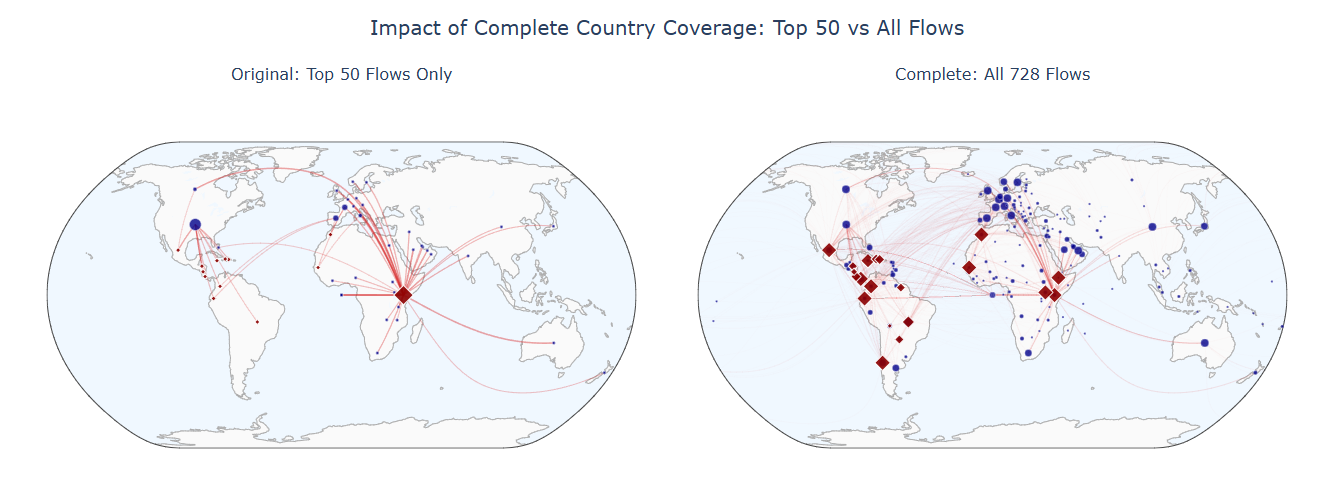
\includegraphics[width=1\textwidth,height=\textheight]{images/9.png}

}

\caption{\label{fig-flow-comparison}Comparison: Main vs Complete Flows}

\end{figure}%

\textbf{Interactive HTML Link}:
\href{https://github.com/WilliamClintC/RER/blob/main/_output/exported_figures/09_comparison_top50_vs_all_flows.html}{View
Interactive Flow Comparison}

\subsection{Key Insights}\label{key-insights}

\subsubsection{Network Structure}\label{network-structure}

\begin{itemize}
\tightlist
\item
  \textbf{Flow Direction}: Strong unidirectional pattern from developed
  to developing nations
\end{itemize}

\section{Appendix}\label{appendix}

\subsection{HTML Interactive Versions of
Graphs}\label{html-interactive-versions-of-graphs}

Please access the HTML files in:
\href{https://github.com/WilliamClintC/RER/tree/main/_output/exported_figures}{\texttt{output\textbackslash{}exported\_figures\textbackslash{}}}


\printbibliography


\end{document}
